\section{Unterraum der Differenzgesichter} \label{sec:facespace}
\begin{tcolorbox}
	\centerline{\textbf{Lernziele Kapitel~\ref{sec:facespace}}}
	\begin{enumerate}[leftmargin=*,label=\thesection.\arabic*]
		\item Den Durchschnitt einer Familie von Vektoren geometrisch \textit{verstehen}.
		\item Die Translation von Punkten um einen Vektor geometrisch \textit{verstehen}.
		\item Den Begriff \glqq{}Unterraum\grqq{} \textit{erklären} können.
		\item Die Begriffe Durchschnittsgesicht, Differenzgesicht \textit{verstehen}.
	\end{enumerate}
\end{tcolorbox}
Seien nun $M,N\in\mathbb N$ fix.
Wir haben im letzten Kapitel gesehen, wie man schwarz-weiss Bilder der Auflösung $M\times N$ als Vektoren in $\mathbb R^{M\cdot N}$ verstehen kann.
Die Bilder müssen dafür nicht unbedingt ein Gesicht zeigen.
Die Pixel können sogar völlig zufällige Graustufen aufweisen, so dass auf dem Bild nichts sinnvolles zu erkennen ist.
Dies führt uns zu folgender Beobachtung:
Nur die wenigsten Vektoren in $\mathbb R^{M\cdot N}$ entsprechen einem Gesicht.
Wir wollen uns näher mit dieser Beobachtung befassen.

Sei $K\in\mathbb N$ die Anzahl aller Bilder von allen Personen unserer Datenbank.
Jedes Bild soll dabei die Auflösung $M\times N$ haben.
Wir betrachten alle Bilder der Datenbank als Vektoren $\vec b_1,\ldots,\vec b_K\in\mathbb R^{M\cdot N}$.
Diese Darstellung erlaubt uns, das \textit{Durchschnittsgesicht}, wir nennen es $\vec m\in\mathbb R^{M\cdot N}$, zu definieren
\begin{equation*}
	\vec m=\frac{1}{K}\left(\vec b_1+\ldots+\vec b_K\right).
\end{equation*}
Das Durchschnittsgesicht lässt sich wieder als Bild ausgeben.
Aber wie sieht so ein Durchschnittsgesicht aus?
Das werden wir in folgender Übung herausfinden.
\begin{aufgabe}
	Ergänzen Sie im File \texttt{eigenfaces.py} die Funktion \texttt{meanface(b\_list)}.
	Dabei ist \texttt{b\_list} die Liste der Länge $K$ der Vektoren $\vec b_1,\ldots,\vec b_K$.
	Der Rückgabewert soll das Durchschnittsgesicht $\vec m$ sein.
	Sie können die ihre Lösung überprüfen indem Sie das Skript \texttt{meanface\_test.py} laufen lassen.
	\textit{Hinweis:} Die Python Funktionen \texttt{len(...) und sum(...)} können nützlich sein.
\end{aufgabe}
\begin{losung*}
	Hier ist eine mögliche Lösung und das davon mit \texttt{meanface\_test.py} generierte Durchschnittsgesicht.\\[0.5cm]
	\begin{minipage}{0.45\textwidth}
\begin{lstlisting}[style=python]
def meanface(b_list):
	K = len(b_list)
	return sum(b_list) / K
\end{lstlisting}
	\end{minipage}\hfill
	\begin{minipage}{0.3\textwidth}\vspace{-1cm}
		\centering\hfill Durchschnittsgesicht:
	\end{minipage}
	\begin{minipage}{0.2\textwidth}\vspace{-1cm}
		\centering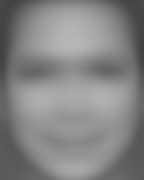
\includegraphics[width=0.6\textwidth]{images/facespace/meanface}
	\end{minipage}
\end{losung*}
Nachdem wir nun das Durchschnittsgesicht gebildet haben, berechnen wir nun die \textit{Differenzgesichter} $\vec a_1,\ldots,\vec a_K$.
Diese sind definiert als
\begin{equation*}
	\vec a_k=\vec b_k-\vec m,\quad k\in\left\{1,\ldots,K\right\}.
\end{equation*}
Die eben eingeführten Begriffe sind links in Abbildung~\ref{fig:meandiff} stark vereinfacht visualisiert.
\begin{figure}[ht]
	\centering
	\begin{minipage}{0.5\textwidth}
		\centering
		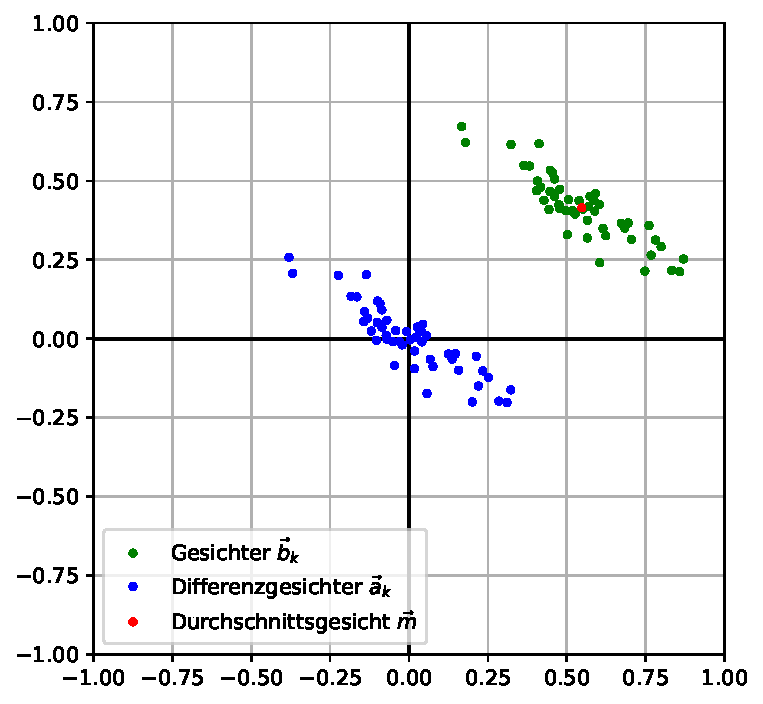
\includegraphics[width=\textwidth]{images/facespace/meandiff}
	\end{minipage}\hfill
	\begin{minipage}{0.5\textwidth}
		\centering
		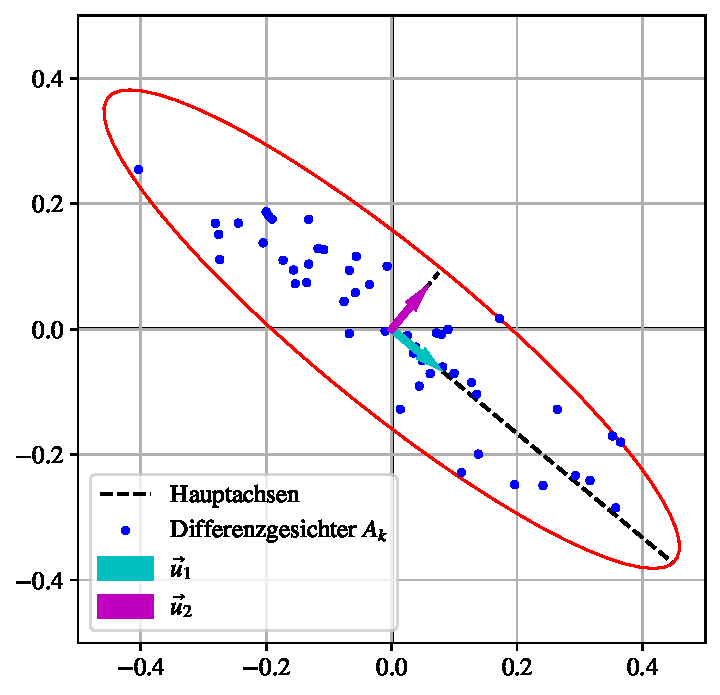
\includegraphics[width=\textwidth]{images/facespace/principal_components}
	\end{minipage}
	\caption{Die Gesichter werden um den Ursprung zentriert indem man das Durchschnittsgesicht subtrahiert (links).
	Die Eigengesichter sind die orthonormalen Vektoren entlang den Hauptachsen (rechts).}
	\label{fig:meandiff}
\end{figure}
\begin{aufgabe}
	Nennen Sie einen Unterschied und eine Gemeinsamkeit der vereinfachten Darstellung links in Abbildung~\ref{fig:meandiff} zu unserer tatsächlichen Situation mit Bildern von Gesichtern.
	Gehen Sie davon aus, dass unsere Bilder eine Auflösung von $M=180$ und $N=144$ haben, wie im letzten Kapitel.
\end{aufgabe}
\begin{losung*}
	Als Vektoren aufgefasst sind die Gesichter Punkte im $\mathbb R^{M\cdot N}$.
	Für $M=180$ und $N=144$ wären das Punkte im $\mathbb R^{25'920}$ und nicht im $\mathbb R^2$ wie in der Abbildung.
	Anders ausgedrückt zeigt die Abbildung den Spezialfall $M\cdot N=2$.
	Das entspricht Bilder die nur aus zwei Pixeln bestehen.
	Andererseits wird in der Abbildung korrekt gezeigt, dass die Komponenten der Gesichts-Vektoren $\vec b_k$ nur Werte zwischen 0 und 1 annehmen.
	Zudem sind die Differenzgesichter richtigerweise genau als Verschiebung der Gesichts-Vektoren um $-\vec m$ dargestellt.
\end{losung*}

Die Eigengesichter werden nun aus den Differenzgesichtern konstruiert.
Wie das genau geht, ist im letzten Kapitel beschrieben.
Hier werden wir nur eine bildliche Konstruktion angeben.
Dazu stelle man sich die Differenzgesichter als eine \glqq{}Wolke\grqq{} von Punkten vor, wie rechts in Abbildung~\ref{fig:meandiff}.
\begin{enumerate}[leftmargin=3cm, label=Schritt \arabic*:]
	\item Entlang einer gewissen Richtung weist diese Wolke die grösste Streuung auf.
	Entlang dieser grössten Streuung wählen wir einen Vektor $\vec u_1$ der Länge 1.
	\item Unter allen Vektoren die orthogonal zu $\vec u_1$ sind, wählen wir wieder einen, der in Richtung der grössten Streuung der Wolke zeigt.
	Diesen nennen wir $\vec u_2$ und er soll wieder Länge 1 haben.
	\item Unter allen Vektoren die orthogonal zu $\vec u_1$ und $\vec u_2$ sind, wählen wir wieder einen, der in Richtung der grössten Streuung der Wolke zeigt.
	Diesen nennen wir $\vec u_3$ und er soll wieder Länge 1 haben.
	\item Analog konstruieren wir $\vec u_4,\vec u_5,\ldots,\vec u_K$.
\end{enumerate}
Die Vektoren $\vec u_1,\ldots,\vec u_K$ heissen \textit{Eigengesichter}.
Sie bilden eine orthonormale Basis des Unterraumes, der von den $K$ Differenzgesichtern aufgespannt wird.
Insbesondere lässt sich jedes der $K$
Wenn man die Komponenten der Eigengesichter geeignet in das Intervall $\left[0,1\right]$ abbildet, lassen sich diese wieder als Bilder darstellen.
%Die Methode der Eigengesichter trifft nun folgende Annahme:
%Die Differenzgesichter sind in guter Approximation in einem niedrig-dimensionalen Unterraum von $\mathbb R^{M\cdot N}$ enthalten.
%Die Dimension dieses Raumes sei $\tilde K$.
%Die obige Annahme bedeutet genauer gesagt, dass $\tilde K\ll K$ und $\tilde K\ll M\cdot N$ (\glqq{}viel kleiner als\grqq{}).
%Wir nennen diesen Unterraum den \textit{Gesichtsraum} (engl. \textit{facespace}).